\chapter{Graphs of Brownian motion}
\label{chap:graphs}

\section{Introduction}
\label{sec:intro-brownian}

Studying the dimension of various random processes has been of interest for quite some time. In this chapter we will consider the Assouad and lower dimensions of graphs of certain random processes, notably L\'evy processes and functions defined by stochastic integrals. Then the regularity dimensions of pushforward measures onto graphs of L\'evy processes will be computed for doubling measures defined on the unit interval. 

In particular we will see that pushforwards of doubling maps in this setting are almost surely not doubling. This contrasts with the previous results on quasisymmetric homeomorphisms which conserved doubling. This will also provide a nice example of a uniformly perfect and doubling space with a non uniformly perfect and non doubling measure fully supported on that same space.

\section{L\'evy processes}
\label{sec:levy-process}


\emph{L\'{e}vy processes} $X(t)$ were first introduced by Paul L\'evy in 1934 \cite{levy} and are defined to be the stochastic processes satisfying:
\begin{itemize}
	\item[1]: $X(0)=0$ almost surely.
	\item[2]: For all $t,h>0$, $X(t+h)-X(t)$ is equal to $X(h)$ in distribution (stationary increments).
	\item[3]: For all $0<t_1<t_2<...<t_k$ the random variables $X(t_i)-X(t_{i-1})$ are independent (independence of increments).
	\item[4]: For all $t>0$ $\lim_{h\to 0} X(t+h)-X(t)=0$ in probability (continuity).
\end{itemize}

We can construct $X(t)$ such that it is almost surely right continuous with left limits (denoted c\`adl\`ag). Such processes are standard tools in many areas of modern mathematics and its applications. A common example of a L\'evy process is the \emph{Wiener process} (or Brownian motion) where property 2 (stationary increments) is replaced by Gaussian increments, so $X(t+h)-X(t)$ is normally distributed with mean 0 and variance $h$. One can similarly define $d$-dimensional Brownian motion by considering the vector-valued stochastic process $(W_1,\ldots, W_d)$ where the $W_i$ are independent Weiner processes. 


\begin{figure}[htbp]
	\centering
	\begin{subfigure}{0.3\textwidth}
		\centering
		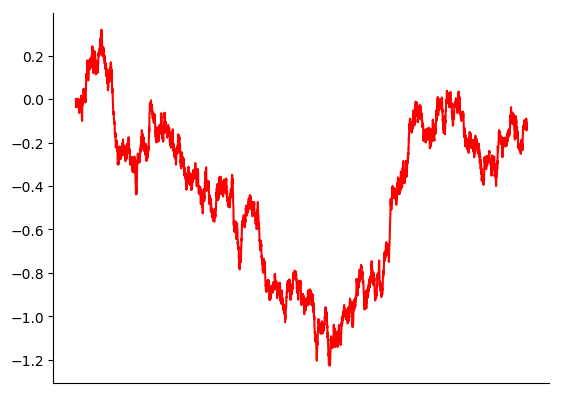
\includegraphics[width=0.85\linewidth]{2-brownianr.png}
	\end{subfigure}%
	\begin{subfigure}{.3\textwidth}
		\centering
		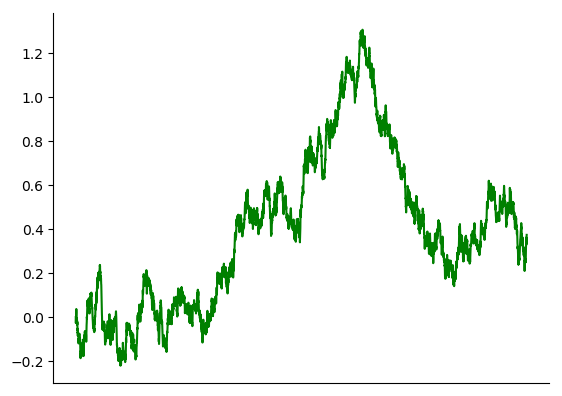
\includegraphics[width=.9\linewidth]{2-browniang.png}
	\end{subfigure}%
	\begin{subfigure}{.3\textwidth}
		\centering
		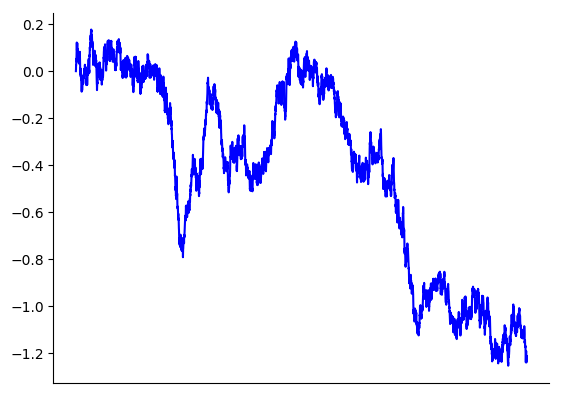
\includegraphics[width=.9\linewidth]{2-brownianb.png}
	\end{subfigure}
	\caption{Three graphs of Brownian motion, a 2-stable L\'evy process.}
	\label{fig:brownian}
\end{figure}



\begin{figure}[h]
	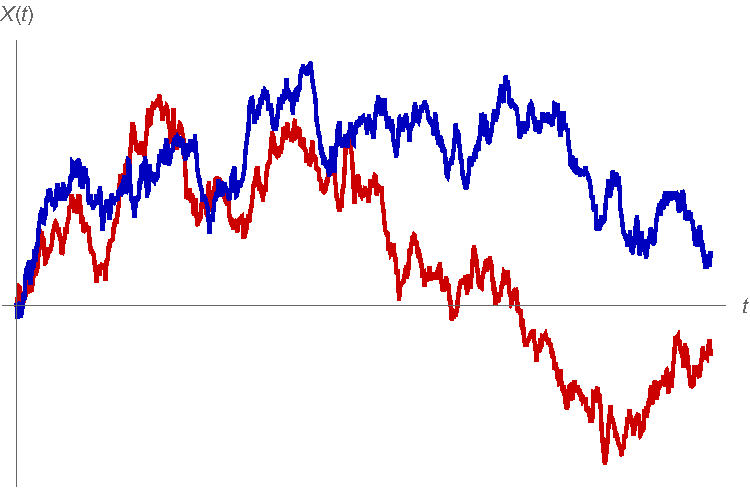
\includegraphics[width=0.5\textwidth]{wiener_process.pdf}
	\caption{\label{fig:brownianmotion}Two graphs of one-dimensional Brownian motion}
\end{figure}

The geometric properties, such as dimension, of Wiener processes have been a particularly well studied area. This includes studying the \emph{graphs}, level sets and \emph{trails} of such processes which can often be thought of as fractals as they often display some \emph{statistical self-affinity}. For any left continuous function $X:\mathbb{R}\to\mathbb{R}$, we define the graph of the function by:
\[
G^{I\subset\mathbb{R}}_{X}=\{(t,y)|y=X(t),t\in I\}\cup J,
\]
where $J$ is the union of vertical segments joining the discontinuities. $J$ is well defined because $X$ is right continuous. It is clear that if $X$ is continuous then $J$ is empty. Taylor \cite{Ta} first calculated the Hausdorff dimension of $d$-dimensional Brownian motion $B_d:\mathbb{R}\to\mathbb{R}^d$ where he showed that almost surely
\[
\dim_\text{H} G_{B_1}^{[0,1]} =  \frac{3}{2}         
\]
and for any $d\ge 2$
\[
\dim_\text{H} B_d([0,1]) =  2.
\]
\textcolor{red}{want to include box dimension result here, equality by kenneth's book}


Another generalisation of Brownian motion is \emph{fractional Brownian motion}, first introduced by Mandelbrot and Van Ness \cite{MVN}. Index-$h$ fractional Brownian motion (fBm) on $\mathbb{R}$ with $0<h<1$ is defined to be the stochastic integral 
\[
B_h (t) = c(h)^{-1} \int_{-\infty}^\infty \left(\left( t-x \right)_+^{h-1/2} - (-x)_+^{h-1/2} \right)W(dx)
\]
where W is the Wiener measure, $(x)_+ = \max\{0,x\}$ and $c(h) = \Gamma(h+1/2)$, where $\Gamma$ denotes the gamma function. Equivalently this is a Gaussian random process $B_h(t)$ with:
\begin{itemize}
	\item[1]: $B_h(0)=0$ almost surely.
	\item[2]: For all $t,u>0$, $B_h(t+u)-B_h(t)$ has normal distribution with mean 0 and variance $u^{2h}$ (Gaussian increments).
	\item[3]: For all $t>0$ $\lim_{u\to 0} B_h(t+u)-B_h(t)=0$ in probability (continuity).
\end{itemize}
One can see that when $h=1/2$, $B_{1/2}(t) = B(t)$ is simply Brownian motion. Much progress has been made on the properties of fBm, see for instance \cite{Ad},\cite{Ka} and \cite{Fa2}. Notably it was shown that almost surely, the graph over the unit interval of index-$h$ fBm has Hausdorff dimension $2-h$. 

\begin{figure}[h]
	\centering
	\begin{subfigure}[b]{0.3\textwidth}
		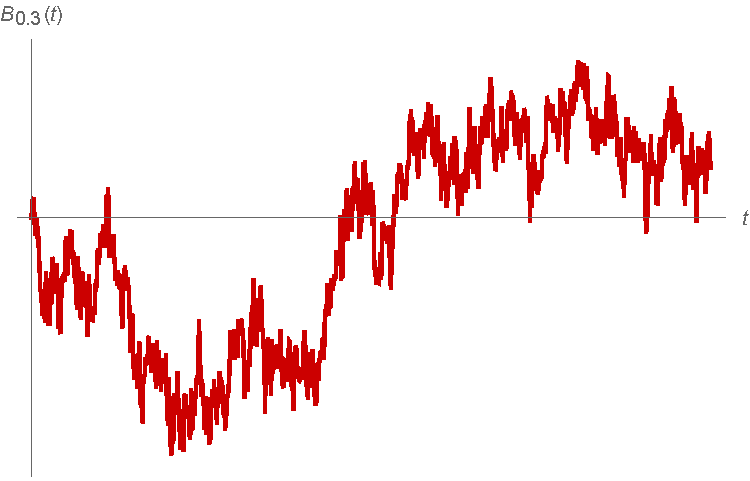
\includegraphics[width=\textwidth]{fbm0_3}
		\caption{Graph of fBm with h=0.3}
		\label{fig:fbm3}
	\end{subfigure}
	~ %add desired spacing between images, e. g. ~, \quad, \qquad, \hfill etc. 
	%(or a blank line to force the subfigure onto a new line)
	\begin{subfigure}[b]{0.3\textwidth}
		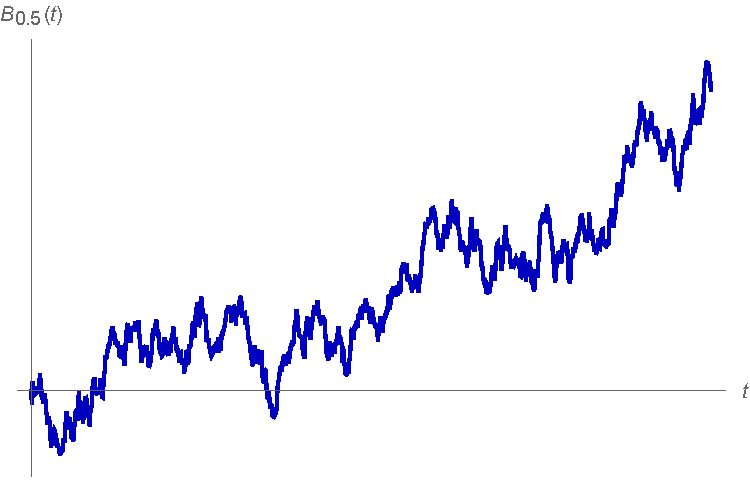
\includegraphics[width=\textwidth]{fbm0_5}
		\caption{Graph of fBm with h=0.5}
		\label{fig:fbm5}
	\end{subfigure}
	~ %add desired spacing between images, e. g. ~, \quad, \qquad, \hfill etc. 
	%(or a blank line to force the subfigure onto a new line)
	\begin{subfigure}[b]{0.3\textwidth}
		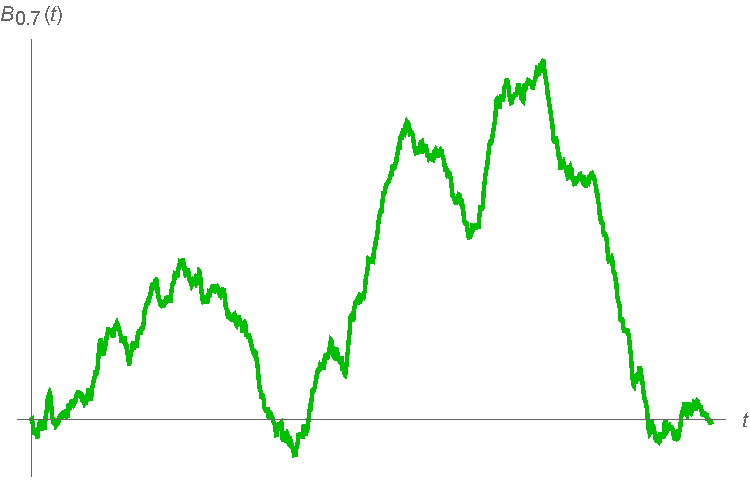
\includegraphics[width=\textwidth]{fbm0_7}
		\caption{Graph of fBm with h=0.7}
		\label{fig:fbm7}
	\end{subfigure}
\end{figure}



Studying the Assouad dimension of various fractals and its properties is an increasingly popular area of research. In this paper, we are interested in calculating the Assouad dimension of the graph $G_X^{[0,1]}$ for $\beta$-scaling (or L\'{e}vy $\beta$-stable) processes and stochastic integrals $X$. These results will be compared to the previously obtained Hausdorff dimensions.

We say that $X(t)$ satisfies a $\beta$-scaling property if, for any $t,a>0$:
\[
a^{-\frac{1}{\beta}}X(at)=^d X(t),
\]
where `$=^d$' denotes `equal in distribution'.
For example the Wiener process has the $2$-scaling property.
The Assouad dimension provides information on the extremal local scaling of a set, in this setting it will tell us about the maximal fluctuations of a random process. For a more detailed introduction to this dimension, see \cite{Fr, Ro}. 

\textcolor{red}{reconfigure whole chapter} This paper will be split into three parts. First we will define a condition, Definition 2.1 which guarantees that a graph will have full Assouad dimension. Then in Section 3 we show that graphs of $\beta$-scaling L\'evy process satisfy this condition and combining these results we prove that graphs of functions defined by certain stochastic integrals also have full Assouad dimension. Finally in Section 4 we remark that our results extend to higher dimensions.

\section{Assouad dimension of graphs}
In this section we will state a convenient condition to check whether a graph of a function $f:[0,1]\to\mathbb{R}$ has full Assouad dimension.

We begin with a definition:

\begin{definition}\label{Win}
	Let $R_1,R_2>0$ be positive numbers and $n_1,n_2>0$ be integers. Given a point $a\in\mathbb{R}^2$, we define $W_{n_1\times n_2}^{R_1\times R_2}(a)$ as the following collection of sets:
	\[	
	\left\{D_{i,j}+a \, \vert \, D_{i,j}=\left[\frac{i}{n_1}R_1,\frac{i+1}{n_1}R_1\right]\times \left[\frac{j}{n_2}R_2,\frac{j+1}{n_2}R_2\right], i\in\{0,\dots,n_1-1\}, j\in\{0,\dots,n_2-1\}\right\}.
	\]
	
	We see that $W_{n_1\times n_2}^{R_1\times R_2}(a)$ is the collection of rectangles with disjoint interiors which partitions the $R_1\times R_2$ rectangle whose bottom left vertex is $a$.
	
	Then let $N_{n_1\times n_2}^{R_1 \times R_2 }(a,G_f^{[0,1]})= \# \left\{ W_{n_1\times n_2}^{R_1\times R_2}(a) \cap G_f^{[0,1]} \right\}$, this is the number of rectangles which intersect the graph.
\end{definition}

The following theorem is a direct consequence of the definition of Assouad dimension and we omit the proof:


\begin{theorem}\label{graph}
	If there exists an $A>0$ and sequences:
	\[
	a_i\in \mathbb{R}^2,R_i\in (0,1),\, n_i\in\mathbb{N} \quad (\forall i\in \mathbb{N})
	\]
	with $n_i \rightarrow \infty$ such that for all $i\in\mathbb{N}$
	\[
	N_{n_i\times n_i}^{R_i \times R_i }(a_i,G_f^{[0,1]})\geq A n_i^2.
	\]
	Then
	\[
	\Assouad G_f^{[0,1]}=2.
	\]
\end{theorem}

Whilst this might seem like a restrictive condition to ask a general function to satisfy, it is quite natural in the setting of Wiener processes due to the almost sure unbounded variation and $\beta$-scaling property of the process. Considering squares instead of balls in the definition of Assouad dimension is similar to the definition of the Furstenberg star dimension, which is in fact equivalent to the Assouad dimenion, see \cite{chenwuwu}.

\begin{remark}
	Note that one could replace the inequality with the following equality
	\[
	N_{n_i\times n_i}^{R_i \times R_i }(a_i,G_f^{[0,1]})= n_i^2.
	\]
	This follows from \cite[Theorem 2.4]{FY}, where it is shown that a set has full Assouad dimension if and only if it has the unit ball as a weak tangent. This means that any cover of our set is also a cover of a ball and so all smaller squares are needed in the cover.
\end{remark}

\section{Applications to  $\beta$-scaling L\'evy processes}\label{LP}

Let $X(t)$ be a L\'evy process. We assume that $X(1)$ is non-vanishing almost everywhere on $\mathbb{R}$ as a random variable, that is, the distribution function of $X(1)$ is 0 only on a set of measure 0. 

Then for any $\beta$-scaling L\'evy process $X$ we can compute the probability of the following event `$N_{n\times n}^{1 \times 1 }(0,G_X^{[0,1]})=n^2$'. It is a positive number depending only on $n$ and we use $P(n)$ to denote this number. The event `$X$ hits a rectangle' is measurable when $X$ is continuous; when it is discontinuous we join the graph with a vertical line and the process is c\`adl\`ag so the event `$X$ hits a rectangle' is still measurable. Thus our event is measurable as the union of measurable events.

For a $\beta$-scaling random process $X$, we can decompose the graph into countably many disjoint parts:
\[
G_X^{[0,1]}=\bigcup_{i=0}^\infty G_X^{I_i},
\]
where $I_i$ are closed intervals with disjoint interiors such that their union is the unit interval. For our case one could think of this as partitioning the unit interval by intervals of length $1/2^i$. For example take $a_1=0$ and for all $i\geq 1$ let $a_{i+1}=a_i+1/2^i$ and $I_i=[a_i,a_i+1/2^{i}].$

Denote by $|I_i|$ the length of interval $I_i=[a_i,b_i]$. Because we can take $X$ as a left continuous function, $X(a_i)\in\mathbb{R}$ is defined for all $i$. For each $i$ we can apply a linear map $T_i: G_X^{I_i} \rightarrow [0,1]^2$:
\[
T_i(x,y)=\left(\frac{1}{|I_i|}(x-a_i),\frac{1}{|I_i|^{1/\beta}}(y-X(a_i))\right).
\]

By definition, it is easy to see that $T_i(G_X^{I_i})$ are independent $\beta$-scaling L\'evy processes with the same, original distribution. For convenience we identify $T_i(G_X^{I_i})=G_{X_i}^{[0,1]}$ where $X_i$  are independent, identically distributed $\beta$-scaling L\'evy processes.

Let $n_i$ be a sequence of integers such that $\lim_{i\to\infty} n_i=\infty$. We can compute the probability of the event $A_i=`N_{n_i\times n_i}^{1 \times 1 }((0,0),G_{X_i}^{[0,1]})=n_i^2 $'. According to the discussions above, we see that the probability is $P(n_i)$. In fact denote $t_k=k/n^2_i$ for all $k\in\{1,\dots,n^2_i\}$ and $D(j)=[j/n_i,(j+1)/n_i]$ for all $j\in\{0,\dots, n_i-1\}$ then we can see that:
\[
P(n_i)\geq P\left(\forall k\in\left[1,n^2_i\right], k\in \mathbb{N},X(t_k)\in D\left(\left\{\frac{k}{n_i}\right\}n_i\right)\right)>0.
\]
Here $\{ \cdot \}$ denotes the fractional part function. The last inequality follows from our assumption that $X(1)$ is non-vanishing almost everywhere on $\mathbb{R}$. It is clear that this restraint could be relaxed to non-vanishing on some interval without much effort. The rest follows from the property of independent increments.

We can choose $n_i$ to grow slowly enough such that $\sum_{i}P(n_i)=\infty$. Note that the $R_i$ can be chosen so that each square is disjoint and as L\'evy processes are Markov, the events $A_i$ are all independent. Then by Borel-Cantelli lemma we see that with probability $1$, infinitely many events $A_i$ occur. Now if $A_i$ happens, then:
\[
N_{n_i\times n_i}^{1 \times 1 }\left((0,0),G_{X_i}^{[0,1]}\right)=n_i^2,
\]
applying the function $T^{-1}_i$ to the graph, we see that (remember $I_i=[a_i,b_i]$):
\[
N_{n_i\times n_i}^{|I_i| \times |I_i|^{1/\beta} }\left((a_i,X(a_i)),G_{X}^{I_i}\right)=n_i^2.
\]

Since $\beta\geq 1$, we see that $|I_i|\leq |I_i|^{1/\beta}$. Also remember that $X$ can be taken to be a right continuous function and we also include the vertical segments of the jumps in $G^{[0,1]}_X$. Therefore it is clear that there exist an absolute constant $C>0$:
\[
N\left(B\left(\left(a_i,X(a_i)\right),|I_i|\right)\cap G_X^{[0,1]},\frac{|I_i|}{n_i}\right)\geq C n_i^2.
\] 

As infinitely many $A_i$ occur, using Theorem \ref{graph}, we see:
\[
\Assouad G_{X}^{[0,1]}=2.
\]

We conclude the above argument as the following theorem:
\begin{theorem}\label{Main}
	Let $X$ be a $\beta$-scaling L\'evy process with $\beta\geq 1$, such that $X(1)$ is a random variable whose distribution function is non-vanishing almost everywhere. Then almost surely:
	\[
	\Assouad G_{X}^{[0,1]}=2.
	\]
\end{theorem}

We know that the Wiener process $W(t)$ is a $2$-scaling L\'evy process, therefore we see that:
\begin{corollary}
	\[
	\Assouad G_{W}^{[0,1]}=2.
	\]
\end{corollary}

Ville Suomala and Changhao Chen, in a personal communication, kindly remarked that this result follows from the graph of Brownian motion having full lower porosity dimension. This approach is inspired by \cite{coxgriffin}, where it was shown that the graph of Brownian motion has full upper porosity dimension. However this porosity dimension technique does not extend to our following, more general result.

In fact we can say more about the Assouad dimension of random processes which are functions defined as stochastic integrals, such as fractal Brownian motion. 

\begin{theorem}
	Let $f:\mathbb{R}\to\mathbb{R}$ be a function which is zero only finitely often, continuous on some interval and has continuous derivative on that same interval. Then we define $B_f(t)$ as the function defined by the stochastic integral:
	\[	
	B_f(t)=\int_0^t f(x) W(dx).
	\]
	We have that almost surely:
	\[
	\Assouad G_{B_f}^{[0,1]}=2.
	\]
\end{theorem}
\begin{remark}
	In particular, graphs of fractional Brownian motions with indices $0<h<1$ have full Assouad dimension almost surely.
\end{remark}
\begin{proof}
	Given a function $f$ which is zero only finitely often, continuous and has continuous derivative on some interval, say $J$, we can simply focus on the function restricted to $J$, normalising to obtain a function which is $C^1$ and zero only finitely often on the unit interval. We may then assume that $f(t)>1$ for $t\in [0,1]$ by again restricting our function to an interval where the function is bounded away from zero and normalising. 
	
	As the Assouad dimension provides local information, if the dimension of the graph of the function defined by stochastic integral of this new function is full then the dimension of the original graph is also full. Thus we assume for the rest of this proof that $f$ is a $C^1$ function which is greater than $1$.
	
	Ideally we would wish to integrate by parts in the standard Riemann–-Stieltjes sense
	\[
	\int_{0}^{t}f(x)W(dx)=f(t)W(t)-\int_{0}^{t}W(x)f'(x)dx.\tag{*}
	\]
	The problem is that the integral on the left side of the above equation is interpreted as the It\^{o} integral, for which regular integration by parts does not hold. There is however a generalisation of this formula for stochastic integrals which holds as $f$ and $W$ are both semimartingales, see \cite{Pr}[Chapter 2 Section 6] for further details. To be precise we should write the following equation
	\[
	\int_{0}^{t}f(x)W(dx)=f(t)W(t)-\int_{0}^{t}W(x)f'(x)dx-[f,W]_t.
	\]
	Here $[f,W]_t$ is the quadratic covariation between $f$ and $W$:
	
	Let $0=t_1<t_2<\dots<t_n=t$ be a partition $P$ of $[0,t]$ and $\vert P \vert$ be the maximum of $t_{k+1}-t_k,k\in\{0,\dots,n-1\}$:
	\[
	[f,W]_t=\lim_{\vert P\vert\to 0} \sum_{i=1}^{n-1} (f(t_{i+1})-f(t_{i}))(W(t_{i+1})-W(t_i)).
	\]
	The above convergence is taken in the sense of probability. By using Cauchy-Schwarz we see that:
	\[
	[f,W]_t\leq [f,f]^{1/2}_t[W,W]^{1/2}_t.
	\]
	However, it is standard that $[f,f]_t=0$ and $[W,W]_t=t$ as $f$ is $C^1$. So we see that the integral by parts formula (*) is indeed correct for this situation. The integral 
	\[
	\int_0^{t} W(x)f'(x)dx
	\]
	is defined to be a random process whose sample space is that of the Wiener process, where fixing a sample path of the Wiener process will determine the integral. We are interested in almost sure properties of this process and will do so by considering almost sure properties of the Wiener process.
	
	The strategy for the rest of this proof is to choose carefully a typical path of the Wiener process. We denote the sample space of the Wiener process as $\Omega$.
	
	First, we see that for almost all $\omega\in\Omega$, $W(t,\omega)$ is c\`adl\`ag in $t$, and therefore there is a constant $C_\omega$ such that:
	\[
	|W(t,\omega)|\leq C_\omega
	\]
	for all $t\in [0,1]$. 
	
	The second almost sure property is described in the proof of Theorem \ref{Main}, that there are infinitely many intervals $I_i=[a_i,b_i]\subset [0,1]$ and a sequence $n_i\to\infty$ such that for $k\in\{0,1,\dots,n_i-1\}$
	\[
	\left|W\left(a_i+(k+1)\frac{|I_i|}{n_i},\omega\right)-W\left(a_i+k\frac{|I_i|}{n_i},\omega\right)\right|\geq |I_i|^{1/2}\geq |I_i|.
	\]
	
	In the following discussion we shall fix a typical $\omega$ such that $W(t,\omega)$ satisfies the above two almost sure properties, in particular, we think of $C_\omega>0$ as a fixed constant.
	
	Then we see that:
	\begin{eqnarray*}
		& &\left|B_f\left(a_i+(k+1)\frac{|I_i|}{n_i},\omega\right)-B_f\left(a_i+k\frac{|I_i|}{n_i},\omega\right)\right|\\
		&=& \left| \int_{a_i+k\frac{|I_i|}{n_i}}^{a_i+(k+1)\frac{|I_i|}{n_i}} f(x)W(dx)\right|\\
		&=& \left| f\left(a_i+k\frac{|I_i|}{n_i}\right)W(x,\omega)\bigg\vert_{a_i+k\frac{|I_i|}{n_i}}^{a_i+(k+1)\frac{|I_i|}{n_i}} + \int_{a_i+k\frac{|I_i|}{n_i}}^{a_i+(k+1)\frac{|I_i|}{n_i}} W(x)f'(x)dx \right|.
	\end{eqnarray*}
	
	Since $f$ is $C^1$, we see that there is a constant $C_f$ (which does not depend on $i$) such that for all $x\in \left[{a_i+k\frac{|I_i|}{n_i}},{a_i+(k+1)\frac{|I_i|}{n_i}}\right]$:
	\[
	\left\vert W(x)f'(x)\right\vert \leq C_f C_\omega.
	\]
	
	Then we have the following inequalities:
	\[
	\left| f\left(a_i+k\frac{|I_i|}{n_i}\right)W(x,\omega)\bigg\vert_{a_i+k\frac{|I_i|}{n_i}}^{a_i+(k+1)\frac{|I_i|}{n_i}} \right| \geq \left| f\left(a_i+k\frac{|I_i|}{n_i}\right) \right| |I_i|^{1/2}\geq |I_i|^{1/2}.\tag{**}
	\]
	and
	\[
	\left\vert\int_{a_i+k\frac{|I_i|}{n_i}}^{a_i+(k+1)\frac{|I_i|}{n_i}} W(x)f'(x)dx \right\vert\leq C_fC_\omega\frac{|I_i|}{n_i}.
	\]
	Since $|I_i|\to 0$,  we see that for a constant $C'$ which depends only on $f$ and $\omega$:
	\[
	\left|B_f\left(a_i+(k+1)\frac{|I_i|}{n_i},\omega\right)-B_f\left(a_i+k\frac{|I_i|}{n_i},\omega\right)\right|\geq C'|I_i|.\tag{***}
	\]
	The above inequality holds for all $k\in\{0,\dots,n_i-1\}$. 
	
	Moreover, $W$ has a `zigzag' property. For even integers $k$ we have
	\[
	W\left(a_i+(k+1)\frac{|I_i|}{n_i},\omega\right)-W\left(a_i+k\frac{|I_i|}{n_i},\omega\right)>0,
	\] 
	for odd integers $k$ we have
	\[
	W\left(a_i+(k+1)\frac{|I_i|}{n_i},\omega\right)-W\left(a_i+k\frac{|I_i|}{n_i},\omega\right)<0.
	\]  
	Heuristically this says that the process increases on the first interval, decreases on the second and so forth, zigzagging from top to bottom. We can see that the expressions inside the absolute values in (**) and (***) also satisfy similar `zigzag' properties. Therefore there is a constant $A=A(\omega,f)>0$ such that:
	\[
	N\left(B\left(\left(a_i,B_f(a_i)\right),|I_i|\right)\cap G_{B_f}^{[0,1]},\frac{|I_i|}{n_i}\right)\geq A n_i^2.
	\] 
	
	This concludes the proof because the above argument holds for a set of full probability $\omega\in\Omega$.
\end{proof}



\section{A remark on higher dimensional Brownian motion}

Definition \ref{Win} has a natural generalization in $\mathbb{R}^d$.
\begin{definition}\label{Win2}
	Let $R_1,\dots,R_d>0$ be positive numbers and $n_1,\dots, n_d$ be integers. Given a point $a\in\mathbb{R}^d$, we define $W_{n_1\times\dots\times n_d}^{R_1\times\dots\times R_d}(a)$ as the following collection of sets:
	\begin{eqnarray*}
		\Bigg\{D_{i_1,\dots,i_d}+a \, \vert \, D_{i_1,\dots,i_d}=\left[\frac{i_1}{n_1}R_1,\frac{i_1+1}{n_1}R_1\right]\times\dots\times \left[\frac{i_d}{n_d}R_d,\frac{i_d+1}{n_d}R_d\right],\\ i_j\in\{0,\dots,n_j-1\}, j\in\{1,\dots,d\}\Bigg\}.
	\end{eqnarray*}
	
	We see that $W_{n_1\times n_2}^{R_1\times R_2}(a)$ is a collection of rectangles with disjoint interiors.
\end{definition}

Using the above definition and a similar argument as the one in section \ref{LP},  Theorem \ref{graph} also extends to higher dimensions, we can show the following result and we omit the proof:

\begin{theorem}
	Let $B_d(t)$ be the $d$ dimensional Brownian motion, from $\mathbb{R}$ to $\mathbb{R}^d$. Then almost surely:
	\[
	\Assouad B_d([0,1])=d.
	\]
\end{theorem}

We can compare this result to the well known \[\dim_{\mathrm{H}} B_d([0,1])=2\] for $d\geq 2$. The Hausdorff dimension being 2 here can be thought as a reflection that higher dimensional Brownian motion is transient, whilst the Assouad dimension shows that there are still areas of maximal fluctuation. 

Brownian motion also provides examples of Salem sets that can have different Hausdorff and Assouad dimensions, we refer the reader to \cite{Ka}  for further discussion on the links between random processes and Salem sets.




\textcolor{red}{do lower dim here}


\textcolor{red}{got some notation to fix wrt previous sections}
\subsection{Pushforwards of measures onto graphs of Brownian motion}


We now turn our attention to pushforwards of measures and ask if doubling and uniform perfectness are preserved in these situations. Specifically we will consider maps from the unit interval onto graphs of L\'evy processes.


Recall the definition of the graph of a L\'evy process $X$ restricted to the unit interval:
\[
G_X^{[0,1]} = \left\{ (t,X(t)) \colon t \in [0,1] \right\}.
\]
More generally, denote by $G_X^I$ the graph of the process $X$ restricted to the interval $I \subseteq [0,1]$. There is a naturally associated map $f: [0,1] \rightarrow \mathbb{R}^2$ which maps the unit interval to the graph of the process, that is $f\colon t \mapsto (t,X(t))$. This will be the map we wish to use to construct pushforward measures, and for the rest of this section $f$ should be assumed to be this map. 

One of the interesting features of L\'evy processes is their statistical self-affinity. Not all processes have this property so we will restrict to \textit{stable} or $\alpha$-\textit{stable processes}, that is for some $\alpha > 0$
\[
a^{-1/\alpha}X(at) =^d X(t)
\]
for all $a,t > 0$ and $=^d$ means equal in distribution. For example the Wiener process is 2-stable. In fact all stable processes have $\alpha \in (0,2]$. 

Our final condition is a simple assumption that the distribution $X(1)$ is non-vanishing on $\mathbb{R}$. Non-zero on an interval would also work, this is just to ensure the graphs are not just multiple flat lines, such as in a Poisson process.


\begin{figure}[htbp]
	\centering
	\begin{subfigure}{0.3\textwidth}
		\centering
		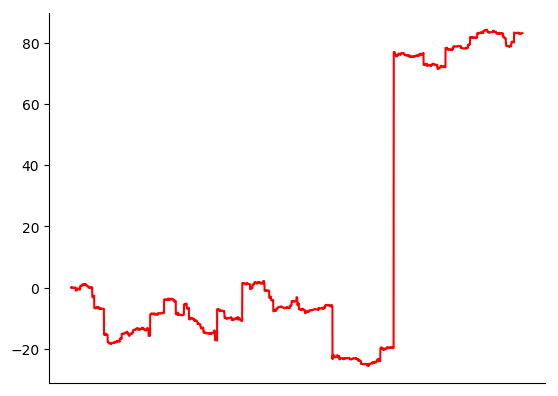
\includegraphics[width=0.85\linewidth]{1-cauchyr.png}
	\end{subfigure}%
	\begin{subfigure}{.3\textwidth}
		\centering
		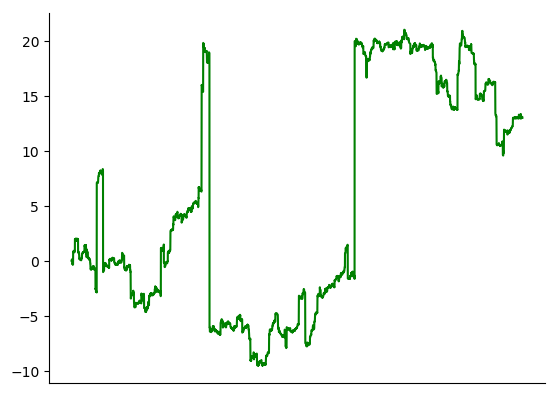
\includegraphics[width=.9\linewidth]{1-cauchyg.png}
	\end{subfigure}%
	\begin{subfigure}{.3\textwidth}
		\centering
		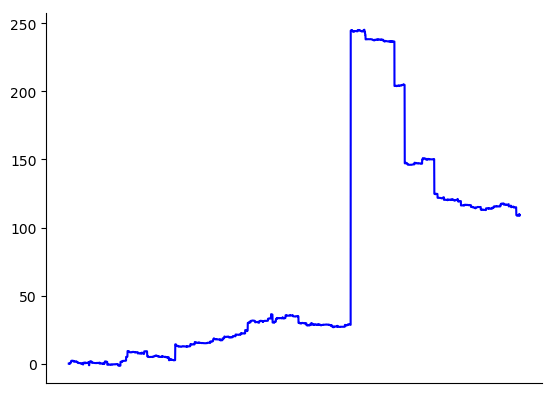
\includegraphics[width=.9\linewidth]{1-cauchyb.png}
	\end{subfigure}
	\caption{Three graphs of a L\'evy process whose increments are Cauchy distributed, a 1-stable L\'evy process.}
	\label{fig:cauchy}
\end{figure}


This leads us to the question of this section: given a doubling measure $\mu$ on the unit interval, is $f_*\mu$ also doubling? A similar question holds for uniformly perfect measures. In \cite{howroyd-yu}, it was shown that the Assouad dimension of $G_X^{[0,1]}$ is almost surely 2 so there must exist at least one doubling measure on the graph. However, most measures on the graph might not even be doubling. For the Hausdorff dimension, the proof by Taylor shows that the Hausdorff dimension of the pushforward of Lebesgue measure almost surely attains the dimension of the graph itself. It turns out that this is usually not the case for the regularity dimensions.

\begin{theorem}\label{brownianthm}
	Let $\mu$ be a doubling measure on $[0,1]$ and $X$ a stable L\'evy process with the distribution $X(1)$ being non vanishing on $\mathbb{R}$. Then $f_*\mu$ is almost surely not doubling on $G_X^{[0,1]}$. Also, $f_*\mu$ is almost surely not uniformly perfect.
\end{theorem}


Trivially this implies the upper regularity dimension of $f_*\mu$ is almost surely infinity and the lower dimension is almost surely zero. Therefore any measure whose upper regularity dimension approximates the dimension of the graph is highly dependent on the specific graph and so there is no one measure that attains the dimension for typical realisations, unlike the Hausdorff case. 


\begin{proof}
    Proof starts here
\end{proof}

Choose a L\'evy process $X$ which satisfies the conditions in Theorem \ref{brownianthm} with scaling coefficient $\alpha$ and fix a graph $G_X^{[0,1]}$ realised by this process. Start by assuming $\alpha > 1$, the proof will work in the same way for $\alpha < 1$ given a slight modification which will be commented on later in the proof. $\mu$ is taken to be a doubling measure on the unit interval. Recall $f$ is defined to be the function which maps the unit interval to the graph of our L\'evy process and $f_*\mu$ is the pushforward measure of $\mu$ onto the graph that we wish to study. \textcolor{red}{properly explain difference when $\alpha < 1$}

We start by calculating the almost sure upper regularity dimension of $f_*\mu$. Let $s>0$. The general strategy for this proof is to find a sequence of events that are all independent and have positive probability. Then a simple application of the Borel-Cantelli lemma will yield that almost surely these events will happen infinitely often. By choosing our events carefully this will yield a sequence of balls that show the upper regularity dimension of the pushforward measure must be greater than $s$. As $s$ is abitrary, this will conclude the proof.

Given our $\alpha$-scaling L\'evy process, we define the rectangle centered at $a\in [0,1]$ with side lengths $R_1,R_2$ by $Rec(a,R_1,R_2) = I(a,R_1) \times I(X(a),R_2)$ where $I(b,R) = [b-R/2,b+R/2]$ is just an interval of length $R$ and centre $b$. $G_X^{I(x,R)}$ will denote the graph of $X$ above the interval $I(x,R)$.

The particular events $E_i$ we are interested in are defined as follows: let $x_i \in [0,1]$, $R_i > r_i> 0$ and $\beta > 1$, then $E_i$ is the event in which $G_X^{I(x_i,R_i^{\alpha})} \subset Rec(x_i,R_i^{\alpha},R_i)$ and $Rec(x_i, r_i, r_i^{1/\alpha}) \cap G_X^{I(x_i,r_i)} = G_X^{I(x_i,r_i^{\beta})}$. These events are chosen so that the measure on the graph will be `large' on the rectangle of small side length $R^{\alpha}$ but `small' on the rectangle of small side length $r$. Figure \ref{brownian_event} is a geometric representation of such an event.  

\begin{figure}[htbp]
	\centering
	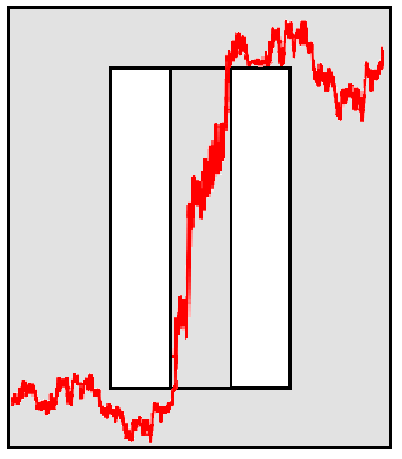
\includegraphics[width=0.4\textwidth]{new_rectangles.png}
	\caption{Example of an event $E_i$, the grey areas are where the graph intersects the rectangles whilst the graph will not intersect the white areas. An example of a graph satisfying this event is in red.}
	\label{brownian_event}
\end{figure}


Note that $\alpha>1$ here is important for the rectangles to be tall and thin. If $\alpha < 1$ it would suffice to change $Rec(x_i,R_i^{\alpha}, R_i)$ to $Rec(x_i, R_i, R^{\alpha})$ and similarly for the smaller rectangles. The rest of the proof would run in the same way afterwards with some slight changes in the calculations of $\beta$ at the end.

Given any sequences $x_i \in [0,1]$, $R_i > r_i > 0$ and $\beta > 1$ we can consider the associated events $E_i$ as above. To make sure the `smaller' rectangle is actually smaller, assume $R_i^{\alpha} > r_i$ without loss of generality. If $Rec(x_m,R_m^{\alpha}, R_m) \cap Rec(x_n,R_n^{\alpha},R_n) = \emptyset$ for all $m\neq n$, then the events are all independent due to the independent increment property of the L\'evy process. As long as the distribution of $X(1)$ is non-vanishing on the unit interval, the probability of any of these events is positive.

We can now choose our sequence of events. Start by picking any disjoint and strictly increasing sequence of reals  $x_i$, $\left\{1-2^{-i} \right\}_{\mathbb{N}}$ would suffice. Then the $R_i$ are taken so that the intervals $I(x_i, R_i)$ do not overlap ensuring independence, say $4^{-i}$. Initially any sequence of $r_i$ can be chosen as long as $R_i/r_i \rightarrow \infty$ and, again, $R_i^{\alpha} > r_i$ for each $i$. $\beta$ will be fixed later, for now it is just a real greater than 1. As the process is $\alpha$-scaling one can map $Rec(x_i,R_i^{\alpha},R_i)$ onto the unit square via an affine map $T$ and the image of the graph under this transformation, denoted $G_{X_i}^{[0,1]}$, will have distribution $X_i$ equal to the original distribution $X(t)$ as it is scaled following the definition of $\alpha$-scaling, so $X(t) = X(R_i^\alpha t)/R_i = X_i(t)$ in distribution. Therefore the probability of an event $E_i$ is equal to the probability the graph of $X_i$ stays in the unit square and 
$$Rec(1/2,r_i/R_i^{\alpha} ,r_i^{1/\alpha}/R_i ) \cap G_{X_i}^{I(1/2, r_i/R_i^{\alpha})} = G_{X_i}^{I(1/2, r_i^{\beta}/R_i^{\alpha})}.$$

Thus the probability of $E_i$ depends solely on the ratio $R_i/r_i = q_i$. If $\sum P(E_i)$ diverges then the conditions for Borel-Cantelli are satisfied and the argument continues. However, if not, the sequence $r_i$ is modified in the following way. Each $i$ gives us a ratio $q_i$ and a probability $P(E_i)$. Construct a function $g \colon \mathbb{N} \rightarrow \mathbb{N}$ such that $g(n) = \lceil \frac{1}{nP(E_n)}\rceil$ for all $n\in \mathbb{N}$. Then, keeping $R_i$ fixed, change the $r_i$ so that each ratio $q_i$ is repeated $g(i)$ many times. For instance, if $g(1) = 3$ then $r_1,r_2$ and $r_3$ are chosen so that $R_1/r_1, R_2/r_2$ and $R_3/r_3$ all give the same $P(E_1)$ and $r_4$ then is chosen with respect to $P(E_2)$ etc. The new sequence is constructed such that $\sum P(E_i)$ diverges, satisfying the conditions for Borel-Cantelli.

Hence, by the Borel-Cantelli lemma, infinitely many $E_i$ occur with probability one. So there are sequences $x_i \in [0,1]$, $R_i > r_i > 0$ and $\beta > 1$ such that, with full probability, all of the events $E_i$ happen and $R_i/r_i \rightarrow \infty$. 

Given a specific event $E_i$ we wish to consider the measure of the rectangles. The ratio of measures of such rectangles is determined by the original measure on the interval. We let $t = \lrdim \mu / 2$, this is just to have a number for which the following bound holds but is also fixed and positive due to Proposition 2.1. Thus we obtain the following bound:
\[
\frac{f_*\mu(Rec(x_i,R_i^{\alpha},R_i))}{f_*\mu(Rec(x_i,r_i,r_i^{1/\alpha}))} = \frac{\mu(B(x_i, R_i^{\alpha}))}{\mu(B(x_i, r_i^{\beta}))} \ge C\left(\frac{R_i^{\alpha}}{r_i^{\beta}}\right)^t, 
\]
where $C$ comes from the definition of the lower regularity dimension.

The only variable left to be fixed is $\beta$. We wish to have the above ratio greater than $C(R_i/r_i)^s$. After a short calculation, it is clear that this is always true if $\beta \ge \alpha + s/t$. Thus by choosing such a $\beta$ we have
\[
\frac{f_*\mu(Rec(x_i,R_i^{\alpha},R_i))}{f_*\mu(Rec(x_i,r_i,r_i^{1/\alpha}))} \ge C\left(\frac{R_i^{\alpha t}}{r_i^{\alpha t + s} }\right) \ge C\left(\frac{R_i^{\alpha t + s}}{r_i^{\alpha t + s} }\right)  \ge
C\left(\frac{R_i}{r_i}\right)^s. 
\]

To show the upper regularity dimension is greater than $s$ we need to consider balls not rectangles. Thankfully due to our construction $B(x_i,R_i) \supset Rec(x_i, R_i^\alpha, R_i)$ and $B(x_i,r_i) \subseteq Rec(x_i, r_i, r_i^{1/\alpha})$. Hence
\[
\frac{f_*\mu(B(x_i,R_i))}{f_*\mu(B(x_i,r_i))} \ge \frac{f_*\mu(Rec(x_i,R_i^{\alpha},R_i))}{f_*\mu(Rec(x_i,r_i,r_i^{1/\alpha}))} \ge C\left(\frac{R_i}{r_i}\right)^s ,
\]
completing the proof.


For the lower regularity dimension it suffices to change the events $E_i$ in the following way. Assuming $\alpha>1$, let $x_i \in [0,1]$, $R_i > r_i > 0$ and $\beta < 1$, then $E_i$ is the event where $G_X^{I(x_i, R_i)} \cap Rec(x_i,R_i,R_i^{1/\alpha}) \subseteq Rec(x_i, r_i^{\beta}, R_i^{1/\alpha})$ and $G_X^{I(x_i, r_i)} \subseteq Rec(x_i, r_i^{\alpha}, r_i)$. The previous argument then works in much the same way, showing that the lower regularity dimension of $f_*\mu$ is zero as desired.

\begin{figure}[htbp]
	\centering
	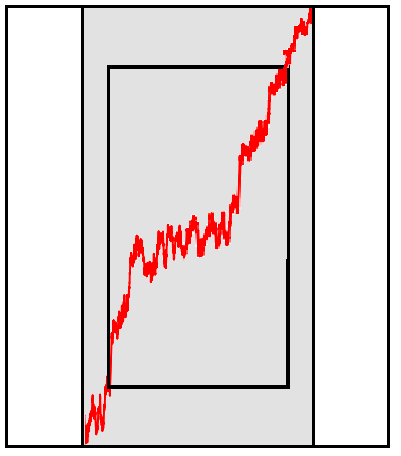
\includegraphics[width=0.4\textwidth]{rectangles.png}
	\caption{Example of an event $E_i$ for the lower regularity dimension, the grey areas are where the graph intersects the rectangles whilst the graph will not intersect the white areas.}
	\label{brownian_event}
\end{figure}






